\documentclass[11pt]{article}
\usepackage[utf8]{inputenc}
\usepackage[T1]{fontenc}
\usepackage{graphicx}
\usepackage{amsmath}
\usepackage{hyperref}
\usepackage{makeidx}
\makeindex

\title{A Texpad Test Document}
\author{Alex}
\date{\today}

\begin{document}
\maketitle
\tableofcontents

\section{Intro}
Hello, world! This is a test of the Texpad workspace. See Live typeset works.
Figure~\ref{fig:plot} and the classic reference \cite{knuth1984}.
LaTeX\index{LaTeX} is a typesetting system.

\begin{equation}
  E = mc^2
  \label{eq:energy}
\end{equation}

\section{A second file}
This section lives in its own file and is pulled in with \verb|\input|.
It tests multi-file structure, tabs and the project file list.

\subsection{Cross-file references}
The energy equation in the main file is Equation~\ref{eq:energy}.


\begin{figure}[htbp]
  \centering
  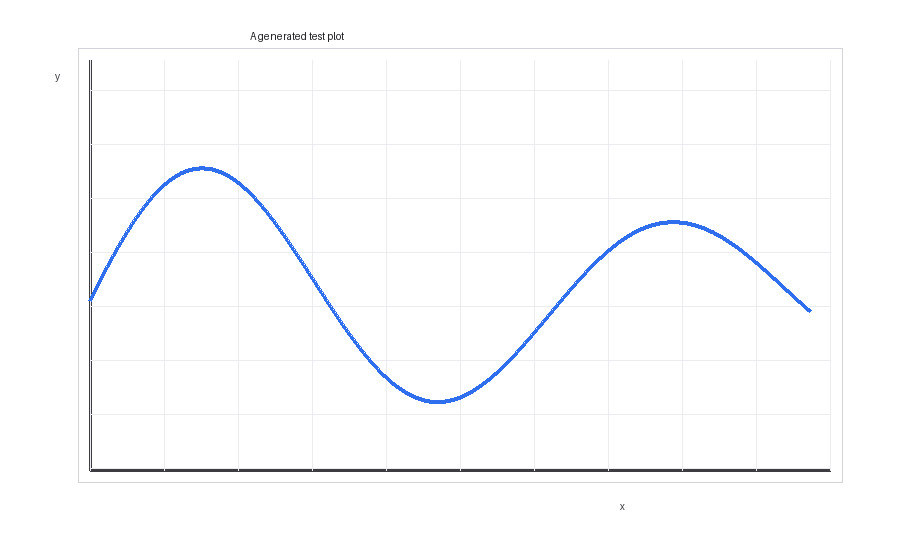
\includegraphics[width=0.55\textwidth]{plot.png}
  \caption{A generated test plot.}
  \label{fig:plot}
\end{figure}

\section{Bibliography test}
According to \cite{knuth1984}, TeX is fun. Lamport's book
\cite{lamport1994} is the standard LaTeX reference.

\bibliographystyle{plain}
\bibliography{refs}

\printindex

\end{document}
